\documentclass{article}
\usepackage[utf8]{inputenc}
\usepackage[english]{babel}
\usepackage{physics}
\usepackage{graphicx}
\usepackage{amsmath}
\usepackage[]{amsthm} %lets us use \begin{proof}
\usepackage[]{amssymb} %gives us the character \varnothing

\title{Advanced Data Analysis\\Homework Week 8}
\author{Aswin Vijay}
\date\today
%This information doesn't actually show up on your document unless you use the make title command below

\begin{document}
\maketitle %This command prints the title based on information entered above

%Section and subsection automatically number unless you put the asterisk next to them.
\section*{Positional Encoding Scheme in "Attention is all you need" Vaswani et al.}
The transformer model architecture proposed in the paper does not 
contain any recurrence or convolutions to encode the order of sequence of the tokens. So 
to encode information about the relative or absolute positions of the input tokens "positional encodings" are
proposed. They are added to the input embedding layer in the encoder and decoder stacks (Figure 1).
\begin{figure*}[h]
    \centering
    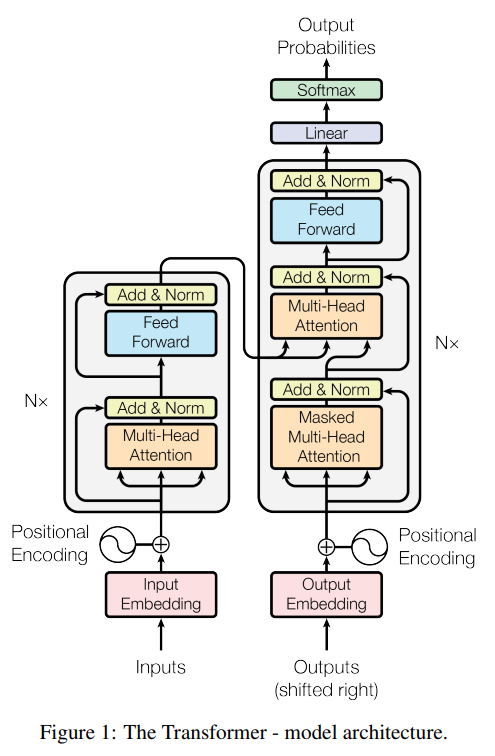
\includegraphics[width=0.35\textwidth]{fig1.png}
\end{figure*} 
The positional encodings used are of the form,
\begin{align*}
    PE_{(pos,2i)} &= \sin(pos/10000^{2i/d_{model}})\\
    PE_{(pos,2i+1)} &= \cos(pos/10000^{2i/d_{model}})
\end{align*}
Where $d_{model}$ is embedding dimension, $pos$ is the position and $i$ is the dimension. The positional embedding
consists of sine and cosine functions of different frequencies. The wavelenghts form a geometric progression and
it was hypothesized that it would allow the model to learn to attend by relative positions as $PE_{pos+k}$ is a linear function of $PE_{pos}$.
It was also hypothesized that the chosen embedding would allow the model to extrapolate to longer sequence lenghts than that encountered during training. 
\end{document}